Esta sección presenta una descripción de los conceptos generales y teóricos en relación con la adquisición de la información de fase, los algoritmos de recuperación de fase y sistemas de clasificación

\subsection{ADQUISICIÓN DE LA INFORMACIÓN DE FASE}

Los sistemas ópticos tradicionales capturan únicamente la información de la intensidad de la luz incidente sobre el sensor, perdiendo con esto la información de fase, que resulta fundamental en aplicaciones como cristalografía de rayos-x \cite{pinilla2018coded}, astronomía \cite{fienup1987phase}, holografía \cite{rivenson2018phase}, entre otras. Por lo tanto, La obtención de la información de  fase  requiere la implementación  de sistemas ópticos que logren codificar la fase de la luz, preservándola implícita en las medidas de intensidad capturadas. 
    
\subsubsection{SISTEMA ÓPTICO DE DIFRACCIÓN}
En múltiples áreas de la ciencia e ingeniería se presenta la captura de medidas de intensidad haciendo uso de sistemas ópticos de difracción\cite{fienup1987phase,pinilla2018coded,rivenson2018phase}. La figura \ref{fig:difraction_systems} muestra un esquema común de los sistemas ópticos de difracción, los cuales se componen por un objeto representado con el vector $\mathbf{z}$ iluminado por luz coherente, modulado en fase por una máscara de fase $\mathbf{D}$, produciendo las medidas cuadráticas codificadas. Dependiendo de la distancia del sensor $L$, la longitud de onda $\lambda$ y el radio de apertura $d$, los modelos de propagación se catalogan en los campos cercano, medio y lejano.

\begin{figure}[H]
    \centering
    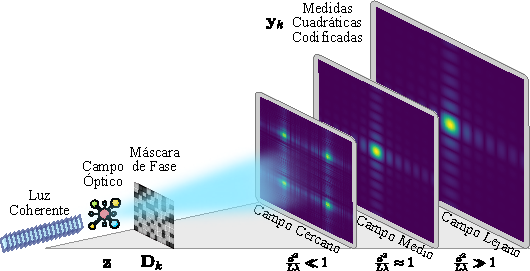
\includegraphics[width=\linewidth]{images/DiffractionSystem.pdf}
    \caption{\hspace{2mm}Sistema óptico codificado de difracción}
    \label{fig:difraction_systems}
\end{figure}

\subsubsection{PROBLEMA DE RECUPERACIÓN DE FASE}

Debido a que los sensores únicamente capturan la información de la intensidad de la luz, el modelo de adquisición se describe como:

\begin{equation}
    \mathbf{y} = \vert \mathbf{A}\mathbf{z} \vert^2, k=1,\dots, m, 
    \label{eq:phase_retrieval_problem}
\end{equation}

Donde $\mathbf{z} \in {\mathbb{C}}^{n}$ es una vectorización del objeto de interés, $\mathbf{y} \in \mathbb{R}^{m}$ son las medidas capturadas y $\mathbf{A}$ es una matriz que describe la propagación del frente de onda de la luz hasta el sensor. De acuerdo con la teoría de difracción\cite{poon2014introduction}, la propagación del frente de onda del objeto se modela entre los campos, cercano, medio y lejano dependiendo del número de Fresnel $F = \frac{d^2}{L\lambda}$, que determina el modelado matemático acorde a la zona de difracción en que se capturan las medidas.

\begin{align}
    \mathbf{y}_k &= \vert \mathbf{FTF}^{H}\mathbf{D}_k\mathbf{z} \vert^2, & \hfill (\text{Campo Cercano, }F \ll 1) \nonumber \\ 
    \mathbf{y}_k &= \vert \mathbf{F}^{H}\mathbf{Q}\mathbf{D}_k\mathbf{z} \vert^2,  & \hfill (\text{Campo Medio, }F \approx 1) \\
    \mathbf{y}_k &= \vert \mathbf{F}\mathbf{D}_k\mathbf{z} \vert^2,  & \hfill (\text{Campo Lejano, } F \gg 1)   \nonumber
    \label{eq:modelado_zonas_difraccion}
\end{align}

Donde $\mathbf{F}$ corresponde a la transformada discreta de Fourier, la matriz diagonal $\mathbf{D}_k \in \mathbb{C}^{n \times n}$ representa el ejemplo $k$ de un conjunto de máscaras de fase donde $k=1,\dots,m$, finalmente $\mathbf{T} \in \mathbb{C}^{n \times n}$ y $\mathbf{Q} \in \mathbb{C}^{n \times n}$ Son matrices ortogonales que modelan la función de transferencia espacial del campo medio y cercano, respectivamente\cite{poon2014introduction,goodman2005introduction}.


\subsubsection{MEDIDAS CUADRÁTICAS CODIFICADAS}
Dado la naturaleza cuadrática de la formulación en la ecuación \ref{eq:phase_retrieval_problem}, este problema se cataloga como NP-difícil. Para mitigar la complejidad, en la literatura, se ha formulado la inclusión de elementos de modulación de fase aleatorios que permitan generar redundancia en las medidas y con esto obtener una solución exacta con alta probabilidad si se tienen las suficientes muestras\cite{candes_CDP}.

las entradas aleatorias de la matriz  $\mathbf{D}_k$ son $i.i.d$ copias de una variable aleatoria $d \in \mathbb{C}$ que satisfacen las siguientes condiciones:

\begin{equation}
    \vert d \vert \leq M, \quad \mathbb{E}[d] = 0, \quad  \mathbb{E}[d^2] = 0, \quad  \mathbb{E}[\vert d \vert^4] = 2\mathbb{E}[\vert d \vert^2]^2    
    \label{eq:restricciones_mascara}
\end{equation}

Donde se busca que $M=1$ puesto que se espera que la codificación no incremente la potencia de las medidas cuadráticas.


\subsection{ALGORITMOS DE RECUPERACIÓN DE FASE}
Para recuperar el campó óptico inicial a partir de medidas cuadráticas codificadas, la literatura ha planteado diferentes algoritmos con formulaciones convexas y no convexas, particularmente, los algoritmos no convexos calculan el gradiente siguiendo la diferenciación de Wirtinger como los mostrados a continuación.

\subsubsection{TRUNCATED WIRTINGER FLOW (TWF)}

El algoritmo TWF propuesto en \cite{chen2017solving}, basa el modelo de muestreo según un variables aleatorias que siguen una distribución de Poisson de la forma:

\begin{equation}
    \mathbf{y}_i \sim Poisson( \vert \langle \mathbf{a}_i,\mathbf{z}\rangle \vert^2 ), \quad i=1,\dots,m
\end{equation}

TWF busca minimizar la máxima estimación de probabilidad 

\begin{equation}
    \minimize_{z \in \mathbb{C}^{n}} - \sum_{i=1}^{m} \ell(\mathbf{z};\mathbf{y}_i)
\end{equation}

Donde $\ell(\mathbf{z};\mathbf{y}_i) = { \mathbf{y}_i log(|\mathbf{a}_i^* \mathbf{z}|^2) -|\mathbf{a}_i^* \mathbf{z}|^2 }$ 

\subsubsection{TRUNCATED AMPLITUDE FLOW (TAF)}

El algoritmo TAF \cite{wang2017solving} adopta un criterio de mínimos cuadrados para recuperar $\mathbf{z}$ basado en las medidas sin fase $\mathbf{y}$ 

\begin{equation}
    \minimize_{\mathbf{z} \in \mathbb{C}^{n}} \frac{1}{m} \sum_{i=1}^{m} (\vert \langle \mathbf{a}_i,\mathbf{z}\rangle \vert - \mathbf{q}_i)^2
\end{equation}

Donde $\mathbf{q}_i = \sqrt{\mathbf{y}_i}$. Este algoritmo asume que las medidas $\mathbf{y}_i$ provienen de un sistema gaussiano de la forma $\mathbf{y}_i \sim \mathcal{N}(\vert \langle \mathbf{a}_i,\mathbf{z}\rangle \vert^2, 1)$

\subsubsection{REWEIGHTED AMPLITUDE FLOW (RAF)}

El algoritmo RAF formulado en \cite{wang2018phase} sigue el criterio de maximizar la estimación de probabilidad de la forma:

\begin{equation}
    \minimize_{z \in \mathbb{C}^{n}} \sum_{i=1}^{m} \ell(\mathbf{z};\mathbf{q}_i/\mathbf{y}_i)
\end{equation}

Donde en el caso de un muestreo con ruido gaussiano basado en la amplitud $\ell(\mathbf{z};\mathbf{y}_i) = (\vert \langle \mathbf{a}_i,\mathbf{z}\rangle \vert - \mathbf{q}_i)^2$ o basado en la intensidad  $\ell(\mathbf{z};\mathbf{y}_i) = (\vert \langle \mathbf{a}_i,\mathbf{z}\rangle \vert^2 - \mathbf{y}_i)^2$. Por otra parte, basado en un muestreo con distribución de Poisson, $\ell(\mathbf{z};\mathbf{y}_i) = { \mathbf{y}_i log(|\mathbf{a}_i^* \mathbf{z}|^2) -|\mathbf{a}_i^* \mathbf{z}|^2 }$ 

\subsection{SISTEMAS DE CLASIFICACIÓN}

La clasificación ha sido una de las tareas computacionales más abordadas en el estado del arte. Específicamente los algoritmos de clasificación se pueden separar en los más tradicionales como las SVM y KNN\cite{kim12012comparing} y los algoritmos basados en redes neuronales que recientemente han dominado diferentes campos\cite{li2019deep,li2018deep, wang2019development}
\subsubsection{CLASIFICADORES TRADICIONALES: SVM, KNN}

\paragraph{máquinas de soporte vectorial (SVM):}

Las máquinas de soporte vectorial(SVM, por su sigla en inglés) \cite{suthaharan2016support} son un método de clasificación binaria, donde cada punto $n$ dimensional $\mathbf{x}_i$ le corresponde una etiqueta de clase $y_i \in \{1,-1\}$.

Suponiendo que los datos de ambas clases son separables linealmente, este método propone separar los datos usando el hiper plano $\mathbf{w}\mathbf{x}_i + b = 0$ de la forma:
\begin{equation}
    \begin{split}
        \mathbf{w}\mathbf{x}_i + b &\geq 1 \quad si \quad y_i=1 \\
        \mathbf{w}\mathbf{x}_i + b &\leq 1 \quad si \quad y_i=-1
    \end{split}
\end{equation}

Resaltando que para todos los elementos del conjunto de datos se cumple que:

\begin{equation}
    y_i(\mathbf{w}\mathbf{x}_i + b) \geq 1, \quad i=1,\dots, m
\end{equation}

El problema de optimización se plantea de la siguiente forma:

\begin{equation}
    \begin{aligned}
        \minimize_{\mathbf{w}} & \quad \Vert \mathbf{w} \Vert \\
        \subjectto_{\quad i=1,\dots, m} & \quad y_i(\mathbf{w}\mathbf{x}_i + b) \geq 1
    \end{aligned}
\end{equation}

Usualmente no es posible separar los datos linealmente, por esta razón se puede incluir una función no lineal $ \phi$ que transforme los datos a un conjunto de características donde las clases sean separables linealmente. El problema de optimización para una SVM usando un kernel $\phi$ se formula como:

\begin{equation}
    \begin{aligned}
        \minimize_{\mathbf{w}} & \quad \Vert \mathbf{w} \Vert \\
        \subjectto_{\quad i=1,\dots, m} & \quad y_i(\mathbf{w}\phi(\mathbf{x}_i) + b) \geq 1
    \end{aligned}
\end{equation}


\paragraph{K vecinos más cercanos (KNN):}

K vecinos más cercanos(KNN, por sus siglas en inglés)Teniendo un conjunto $D = \{(\mathbf{x}_i, y_i)\}_1^n$, siendo $\mathbf{x}_i$ el vector de características e $y_i$ la clase correspondiente. Para un nuevo vector a clasificar $\mathbf{\hat{x}}$, el algoritmo KNN encuentra los $K$ puntos más cercanos del dataset. Usualmente la función de distancia usada usada corresponde a la distancia euclidiana

\begin{equation}
    d(\mathbf{x}_p,\mathbf{x}_q) = \Vert \mathbf{x}_p-\mathbf{x}_q \Vert_2
    \label{eq:distancia_euclidiana}
\end{equation}

Posteriormente haciendo uso de las clases de los $K$ puntos encontrados, de tal forma que $Y \subset D$ y $\vert Y \vert = K$, se cuantifica la cantidad de veces que aparece cada clase y se clasifica la nueva muestra $\mathbf{\hat{x}}$ con la clase que más veces aparezca de la forma

\begin{equation}
    clase(\mathbf{\hat{x}}) =  \argmax_{\hat{y}} \bigg\{ \sum_{y \in Y} \delta(y,\hat{y})\bigg\}
\end{equation}

Donde $\delta(\cdot,\cdot)$ corresponde a la función delta de Kronecker, tal que $\delta(a,b) = 1$ si $a=b$


\subsubsection{CLASIFICACIÓN CON REDES NEURONALES}

Los enfoques de aprendizaje profundo han generado un gran progreso en problemas muy complejos en los últimos años
\cite{he2016deep,li2019deep,li2018deep, wang2019development,wu2016google}. El aprendizaje profundo busca encontrar una función $f: \mathbb{R}^{d_1} \rightarrow \mathbb{R}^{d_2}$. La función $f$ se suele llamar arquitectura de redes neuronal profunda, puesto que consiste en la concatenación de múltiples capas compuestas de unidades mínimas llamadas neuronas. Cada neurona realiza una combinación lineal entre las entradas, para posteriormente usar una función no lineal en la salida. Las salidas de cada neurona en una capa funcionan como entrada de las neuronas ubicadas en la siguiente capa, creando así, una arquitectura de red neuronal profunda \cite{fan2019selective}. 

\begin{equation}
    \footnotesize 
    \big\{f_\theta(\mathbf{x}) = \sigma_{L}(\mathbf{W}_{L}\sigma_{L-1}(\mathbf{W}_{L-1} (\dots \sigma_2(\mathbf{W}_2\sigma_1(\mathbf{W}_1\mathbf{x})))) \quad \vert \quad\theta = \{\mathbf{W}_{1} \dots \mathbf{W}_{L}\}  \big\}
\end{equation}

Donde para cada capa $1 \leq \ell \leq L$, $\sigma_\ell$ corresponde a una función no lineal en dicha capa y $\mathbf{W}_\ell$ La matriz de pesos. Para entrenar los pesos $\theta$ bajo un enfoque de aprendizaje supervisado, este método hace uso de un conjunto de entrenamiento $\{(\mathbf{x}_i, y_i) \}_{i=1}^{N}$ y una función de costo $\mathcal{L}( y_i,  f_\theta(\mathbf{x}_i))$ para plantear el problema de optimización

\begin{equation}
    \minimize_\theta \frac{1}{N}\sum_{i=1}^{N} \mathcal{L}( y_i,  f_\theta(\mathbf{x}_i))
\end{equation}

\subsubsection{CLASIFICACIÓN USANDO MEDIDAS CUADRÁTICAS}
\pagebreak